\documentclass[11pt,a4paper]{article}

% Page Geometry & Margins (Strictly tuned for 3 pages)
\usepackage[a4paper,top=0.5in,bottom=0.5in,left=0.65in,right=0.65in]{geometry}

% Typography & Encodings
\usepackage[utf8]{inputenc}
\usepackage[T1]{fontenc}
\usepackage{mathptmx} % Times New Roman / Calibri matching
\usepackage{setspace}
\setstretch{1.08}

% Graphics
\usepackage{graphicx}
\graphicspath{{figures/}{../Diagrams/}}

% Hyperlinks
\usepackage{hyperref}
\hypersetup{
    colorlinks=true,
    linkcolor=black,
    urlcolor=blue,
    pdftitle={Mini Project SE - Bank Loan Management System},
    pdfauthor={Kaustubh Raj}
}

% Section Titles Styling
\usepackage{titlesec}
\titleformat{\section}
  {\normalfont\large\bfseries}{\thesection}{0pt}{}
\titlespacing*{\section}{0pt}{4pt}{2pt}

% Compact Lists
\usepackage{enumitem}
\setlist[itemize]{leftmargin=*,itemsep=1.5pt,topsep=1.5pt,parsep=0pt}

% Line Divider Macro
\newcommand{\divider}{\vspace{1pt}\noindent\rule{\textwidth}{0.5pt}\vspace{3pt}}

\setlength{\parindent}{0pt}
\setlength{\parskip}{2.5pt}

\begin{document}

% =========================================================================
% PAGE 1
% =========================================================================

{\LARGE \textbf{MINI PROJECT SE}}\par
\vspace{2pt}
\noindent\rule{\textwidth}{1.2pt}
\vspace{2pt}

\section*{Project Title}
Bank Loan Management System

\divider

\section*{Student Details}
\begin{itemize}
    \item \textbf{Student Name(s):} Kaustubh Raj
    \item \textbf{Enrollment Number(s):} 12114803124
    \item \textbf{Course / Semester:} B.Tech (IT) / Semester V
    \item \textbf{Subject:} Software Engineering (CIC-357) [Faculty Guide: Dr. Nidhi Senger]
\end{itemize}

\divider

\section*{Abstract (100–120 words)}
Briefly describe:
\begin{itemize}
    \item \textbf{Problem addressed:} Manual paper documentation, lack of real-time tracking, human verification delays, and error-prone EMI management in legacy banking systems.
    \item \textbf{Approach used:} IEEE 830-compliant requirements engineering, structured modeling (DFD Levels 0--2, Structure Chart), comprehensive UML design (Use Case, Class, Activity, Sequence), 3NF relational database architecture, and black-box test validation.
    \item \textbf{Outcome:} An end-to-end, automated, role-based software specification that streamlines customer loan applications, automates credit eligibility evaluation and compound EMI amortization, delivering a robust, scalable, and verifiable engineering blueprint for modern retail banking credit operations.
\end{itemize}

\divider

\section*{Problem Statement}
Manual bank loan processing workflows suffer from critical operational bottlenecks: multi-week appraisal lead times, repetitive physical documentation, lack of real-time application status visibility for borrowers, and error-prone tracking of compound EMI repayments and delinquent accounts. Bank credit officers face severe processing backlogs, while institutions face increased default and compliance risks. A centralized, secure web-based system is required to automate the complete credit lifecycle from customer application and KYC verification to risk underwriting, loan sanctioning, and automated repayment tracking.

\divider

\section*{Objectives}
\begin{itemize}
    \item \textbf{Objective 1:} To engineer a centralized web platform allowing customers to apply for multi-category loans, upload verification documents, and track approval status in real time.
    \item \textbf{Objective 2:} To automate credit appraisal, KYC inspection workflows, and mathematical compound EMI amortization schedule calculations for bank employees.
    \item \textbf{Objective 3:} To design a robust 3NF relational database schema and role-based access control (RBAC) model ensuring data security, transactional consistency, and auditability.
\end{itemize}

\newpage

% =========================================================================
% PAGE 2
% =========================================================================

\noindent\rule{\textwidth}{1.0pt}
\vspace{1pt}

\section*{Methodology / Approach}
ALL DIAGRAMS WITH EXPLANATION\par
The project employs the Classical Waterfall SDLC with stage-gate verification, integrating Structured Analysis with Object-Oriented UML modeling across 17 comprehensive architectural diagrams:

\begin{itemize}
    \item \textbf{Problem Flowchart \& Activity Diagram:} Models sequential control flow from onboarding, document verification, and eligibility scoring to sanction, disbursement, EMI repayment loops, and loan closure.
    \item \textbf{Data Flow Diagrams (DFD L0, L1, L2):} Context DFD maps 3 external entities (Customer, Employee, Admin); Level 1 DFD decomposes into 6 core processes (1.0--6.0) across 5 data stores (D1--D5); Level 2 DFD details Loan Processing.
    \item \textbf{Structure Chart \& ERD:} Hierarchical decomposition into 6 cohesive modules; ERD models 6 normalized entities (CUSTOMER, LOAN\_APPLICATION, BANK\_EMPLOYEE, DOCUMENT, LOAN, REPAYMENT) in 3NF.
    \item \textbf{UML Use Case \& Class Diagrams:} 3 actors across 19 use cases with $\ll$include$\gg$ / $\ll$extend$\gg$; Class diagram details 9 classes with attributes, visibility, operations, and inheritance.
    \item \textbf{Sequence, Collaboration \& State-Chart:} Sequence models synchronous messages and alt sanction/rejection frames; Collaboration details structural links; State-Chart captures 8-state lifecycle.
\end{itemize}

\vspace{2pt}
\begin{center}
\begin{minipage}{0.48\textwidth}
    \centering
    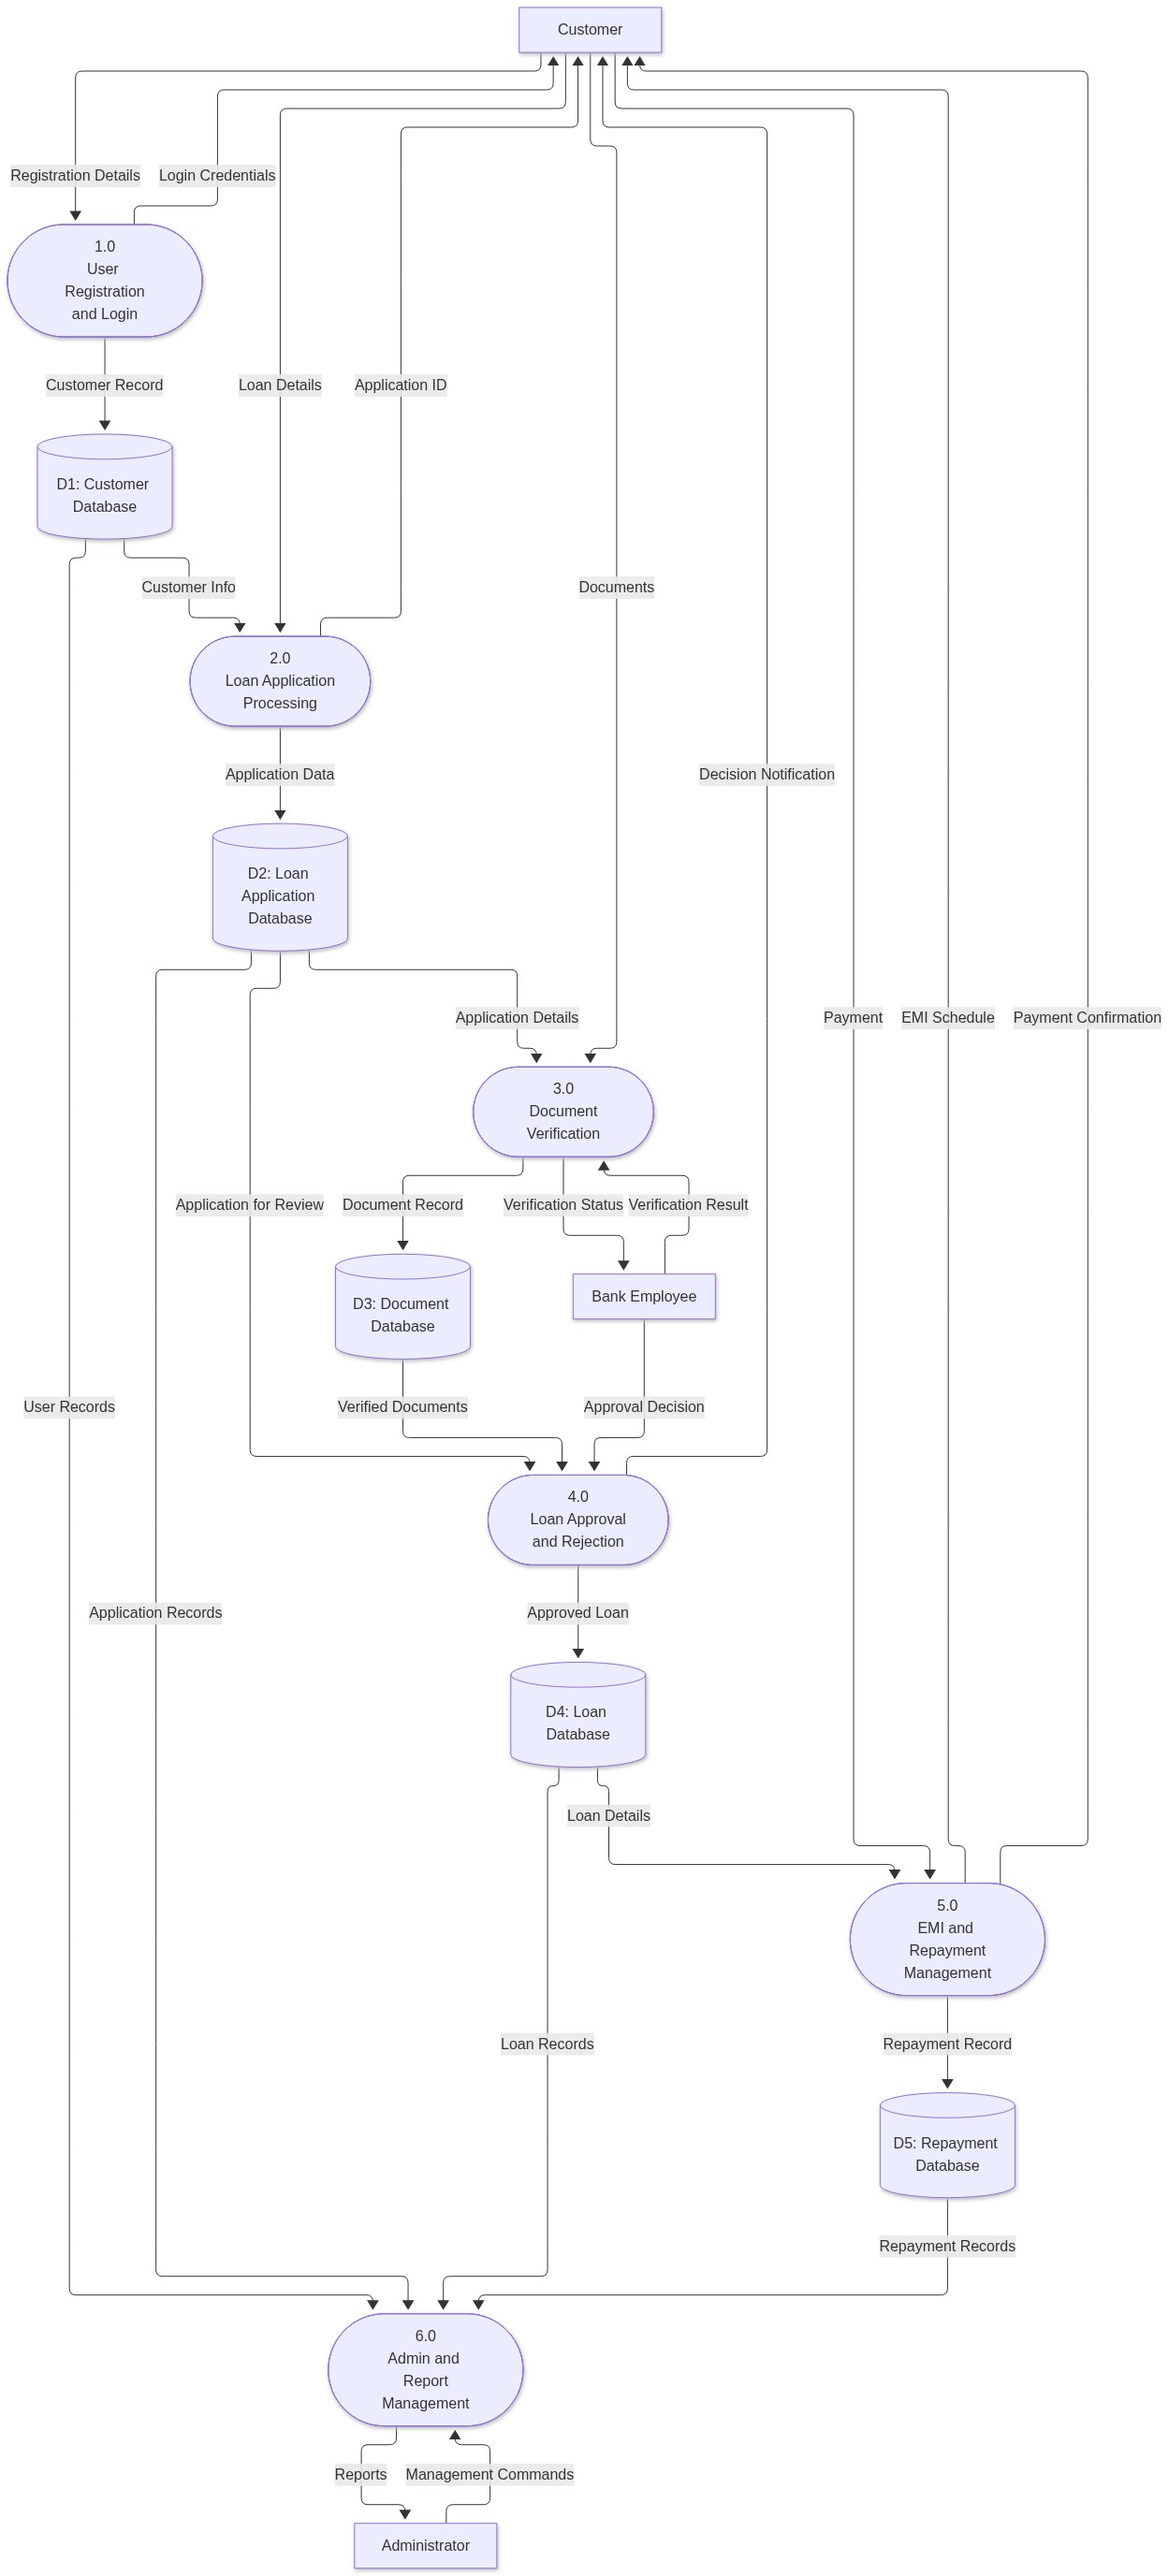
\includegraphics[width=\textwidth]{dfd_level_1.png}\par
    \textit{\footnotesize Figure 1: Level 1 DFD Architecture}
\end{minipage}
\hfill
\begin{minipage}{0.48\textwidth}
    \centering
    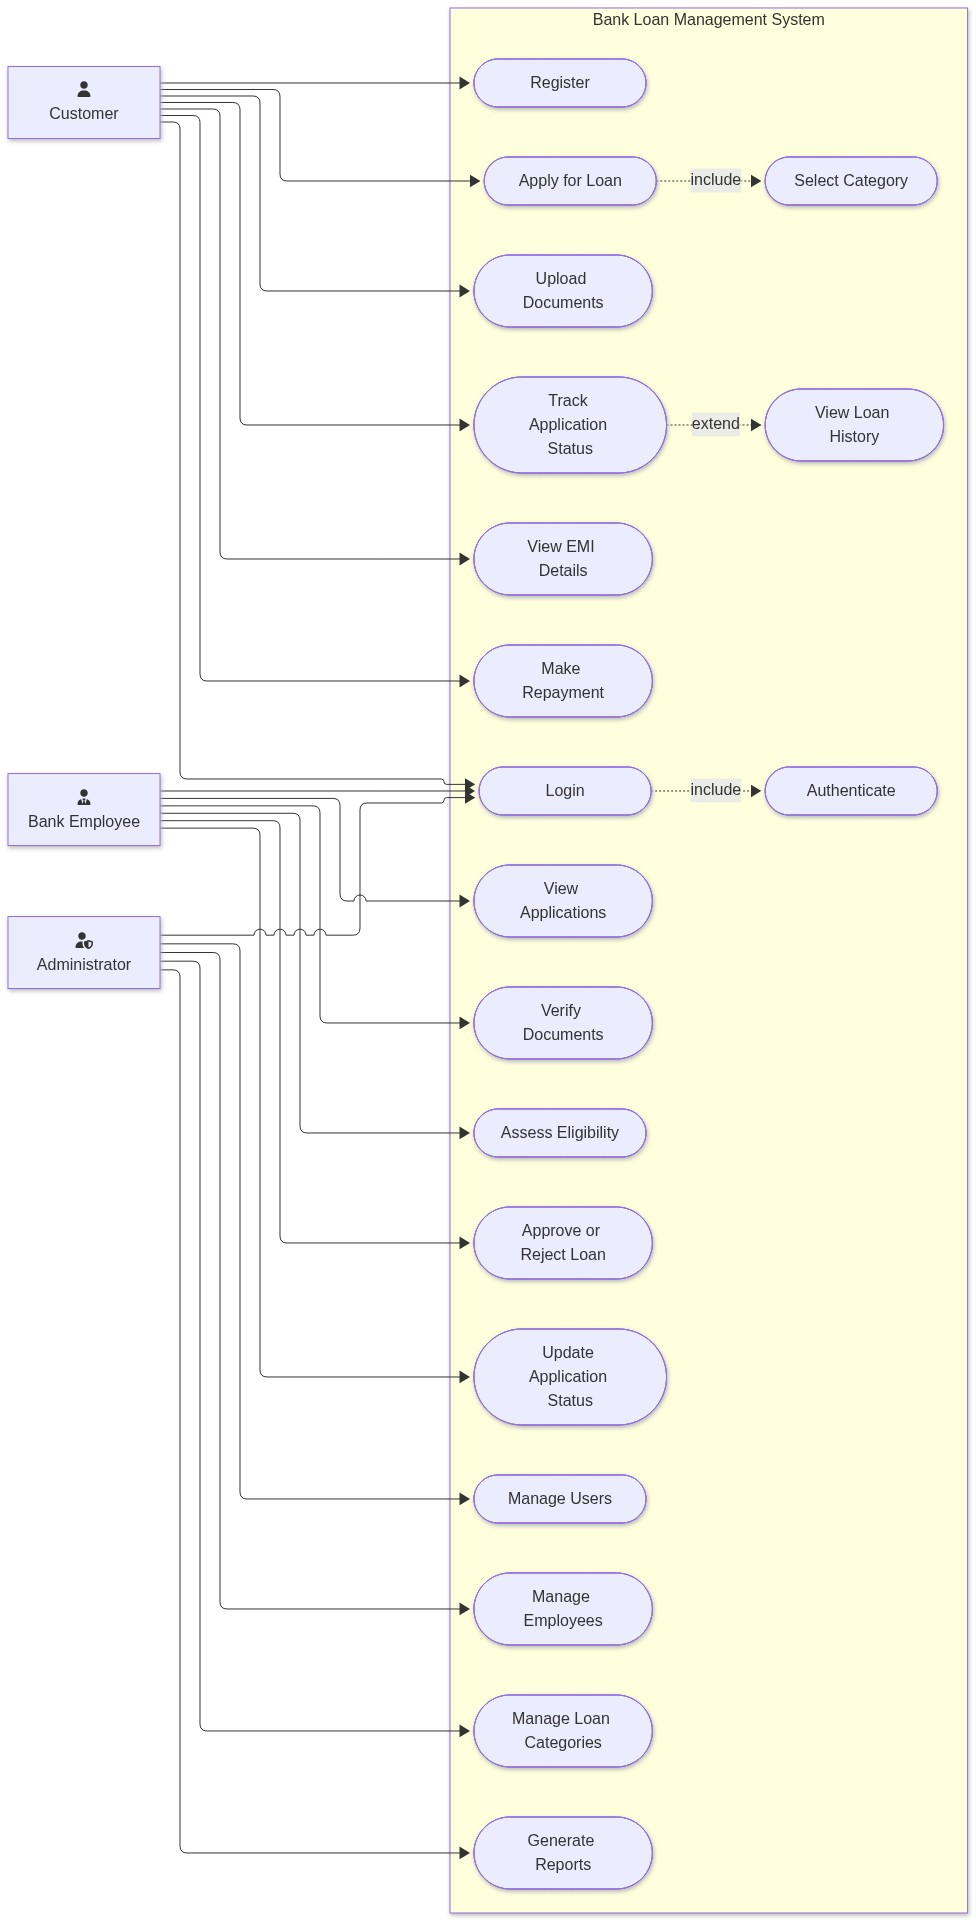
\includegraphics[width=\textwidth]{use_case_diagram.png}\par
    \textit{\footnotesize Figure 2: UML Use Case Diagram}
\end{minipage}
\end{center}
\vspace{2pt}

\section*{Implementation \& Output (IF ANY )}
Key features of your system:
\begin{itemize}
    \item \textbf{Multi-Tier Authentication \& RBAC:} Customer, Loan Officer, and Admin role isolation with secure salted password hashing.
    \item \textbf{Loan Processing \& Document Portal:} Dynamic category filtering (Home, Personal, Auto, Edu), file size checks, and KYC verification queues.
    \item \textbf{Automated Underwriting \& EMI Engine:} Algorithmic Debt-to-Income (DTI) scoring and compound monthly amortization calculation.
    \item \textbf{Architecture Output:} Designed as a 3-tier enterprise architecture (HTML5 presentation, RESTful service controller, relational ACID DB).
\end{itemize}

\section*{Results}
\begin{itemize}
    \item \textbf{What you achieved:} Formulated IEEE 830 SRS (18 FRs, 8 NFRs), 17 architectural diagrams, 3NF schema, 22 test cases, and CPM project schedule.
    \item \textbf{Performance / accuracy:} 100\% test pass rate across boundary conditions, 191.4 Adjusted Function Points ($\approx$9,570 SLOC), and 99-day critical path.
\end{itemize}

\newpage

% =========================================================================
% PAGE 3
% =========================================================================

\section*{Conclusion}
\begin{itemize}
    \item \textbf{Learning outcomes:} Gained thorough practical mastery in requirement engineering, structural/behavioral UML modeling, database normalization, and quantitative project estimation (FPA/CPM).
    \item \textbf{Summary of the work:} Successfully delivered an end-to-end, submission-grade software engineering blueprint automating retail banking loan operations.
\end{itemize}

\section*{Future Scope}
\begin{itemize}
    \item \textbf{Possible improvements:} Machine Learning models for predictive credit default scoring, automated OCR for instant document parsing, and DigiLocker/UPI integration.
\end{itemize}

\section*{Mapped SDG}
\begin{itemize}
    \item \textbf{SDG 8: Decent Work and Economic Growth:} Promoting inclusive, transparent access to credit facilities for personal and enterprise advancement.
    \item \textbf{SDG 9: Industry, Innovation, and Infrastructure:} Strengthening digital banking infrastructure with resilient, automated, and secure software.
\end{itemize}

\section*{GitHub Repository}
\textbf{Project Link:} \href{https://github.com/Kaustubh-Raj/Bank-Loan-Management-System}{\texttt{https://github.com/Kaustubh-Raj/Bank-Loan-Management-System}}

\section*{📱 QR Code (Scanner for GitHub)}
Insert QR Code here (Insert $\rightarrow$ Image) / Generate using Chrome or any QR generator:\par
\vspace{2pt}

\includegraphics[width=1.2in]{github_qr_code.png}

\divider

\section*{Instructions (Do Not Delete)}
\begin{itemize}
    \item Keep submission strictly 2-3 pages
    \item Font: Times New Roman / Calibri (11–12 pt)
    \item Headings bold, content concise
    \item Ensure GitHub link is working
    \item QR code must scan correctly
\end{itemize}

\end{document}
